\documentclass[11pt,a4paper]{article}

% ------------------------------------------------------------------ packages
\usepackage[margin=1in]{geometry}
\usepackage[T1]{fontenc}
\usepackage{lmodern}
\usepackage{microtype}
\usepackage{amsmath,amssymb,amsthm}
\usepackage{graphicx}
\usepackage{booktabs}
\usepackage{multirow}
\usepackage{xcolor}
\usepackage{tikz}
\usetikzlibrary{positioning,arrows.meta,fit,calc,backgrounds}
\usepackage{enumitem}
\usepackage{xspace}
\usepackage{caption}
\usepackage{subcaption}
\usepackage[numbers,sort&compress]{natbib}
\usepackage[colorlinks=true,linkcolor=blue!60!black,citecolor=blue!60!black,urlcolor=blue!60!black]{hyperref}
\usepackage[capitalise,noabbrev]{cleveref}

\setlist{itemsep=2pt,topsep=3pt}
\captionsetup{font=small,labelfont=bf}

% >>> Replace with your repository URL before submitting <<<
\newcommand{\repourl}{https://github.com/Prathamkogta/Lore_Personalisation_Study}

\newcommand{\R}{\mathbb{R}}
\newcommand{\simplex}{\Delta^{K-1}}
\newcommand{\pp}{\,pp\xspace}
\definecolor{lorecol}{HTML}{EB6834}
\definecolor{basecol}{HTML}{2A78D6}

\title{\vspace{-1.2cm}\textbf{Where does LoRe's personalisation come from?}\\[2pt]
\large Stress-testing the basis, the function class and the few-shot step\\ of low-rank reward models}
\author{
\begin{tabular}{c}
DA5453 Learning From Human Preference --- Course Project Report\\[4pt]
\textbf{Pratham Kogta} (ED22B020) \qquad \textbf{B S Tejas} (ED22B004)
\end{tabular}}
\date{November 2026}

\begin{document}
\maketitle
\vspace{-0.6cm}
\begin{center}
\small Paper studied: A.~Bose, Z.~Xiong, Y.~Chi, S.~S.~Du, L.~Xiao, M.~Fazel,
\emph{LoRe: Personalizing LLMs via Low-Rank Reward Modeling}, arXiv:2504.14439 (2025).\\
Code, results, paper and our presentation slides: \url{\repourl}
\end{center}


\begin{abstract}
\noindent LoRe models each user's reward as a mixture of a few shared basis reward functions, learned
as a linear map on frozen reward-model embeddings. A new user is then fitted from a handful of
comparisons by learning only their mixture weights. We first reproduce LoRe on PersonalLLM and Reddit
TL;DR, landing within 0.4--2.2 percentage points (pp) of the paper. We then run two experiments. In the
first, we replace LoRe's linear basis with eight alternatives, from frozen PCA directions to small
MLPs. The linear basis turns out to be essentially sufficient: richer bases add at most 0.6\pp on the
semi-synthetic benchmark and nothing on real users. In the second, we start new users from the
learned seen-user population instead of LoRe's random initialisation. This helps a lot early on: picking
the best-matching seen user, with no gradient steps at all, already matches 50 steps of LoRe's
few-shot training.
\end{abstract}

% ======================================================================
\section{Background: the ideas behind LoRe}
\label{sec:background}

\paragraph{Learning a reward from comparisons.} Reward models for RLHF are trained on pairwise
comparisons: for a prompt $x$, an annotator says that response $y_c$ is better than $y_r$. The
Bradley--Terry (BT) model \citep{bradley1952rank,christiano2017deep} assumes a scalar reward $r(x,y)$ and
sets $P(y_c\succ y_r\mid x)=\sigma\big(r(x,y_c)-r(x,y_r)\big)$, so the reward is learned by minimising the
logistic loss $\ell(z)=\log(1+e^{-z})$ on the reward margin. Standard RLHF fits \emph{one} such reward to
everyone's comparisons. When annotators genuinely disagree (one prefers short answers, another
detailed ones), a single reward averages them, and the result represents nobody in particular.

\paragraph{Idea 1: preferences decompose into a few basis rewards.} LoRe's central assumption is
that people's preferences differ, but not arbitrarily. Most of the variation can be explained by a
small number of underlying criteria, for example helpfulness, conciseness, formality or safety. LoRe
therefore learns $K$ \emph{basis} reward functions $R_\phi(x,y)\in\R^K$ that are shared by everybody, and
writes each user's reward as a weighted combination of them:
\[
r_i(x,y)=w_i^\top R_\phi(x,y),\qquad w_i\in\simplex .
\]
A user is now just a point $w_i$ on the simplex: a set of $K$ non-negative weights that sum to one,
which can be read as ``how much this person cares about each criterion''. All users' rewards then
lie in the same $K$-dimensional space. This is what makes the model \emph{low-rank}.

\paragraph{Idea 2: collaborative ranking.} The same idea powers recommender systems
\citep{koren2009matrix,park2015preference}. In a Netflix-style user$\times$movie rating matrix,
people's tastes are correlated, so the matrix is approximately low-rank. It factorises as
(user factors)$\times$(movie factors), and a new user's ratings can be predicted from a few of their
ratings, because their factor vector is all that is unknown. LoRe applies this to language models. The
``items'' are responses, of which there are infinitely many, so instead of storing one factor per item
it \emph{parameterises} the item factors with a function of the response: $R_\phi(x,y)=A\,e(x,y)$. Here
$e(x,y)\in\R^{4096}$ is the frozen final-token embedding of a pre-trained reward model and
$A\in\R^{K\times4096}$ is learned.

\paragraph{Idea 3: share the basis, personalise cheaply.} Because the basis is shared, it can be
learned from many users at once. A new user then only needs $K$ numbers, which can be estimated from a
handful of comparisons. With $\Delta=e(x,y_c)-e(x,y_r)$, LoRe trains in two stages:
\begin{align}
\text{(1) seen users:}\quad &\min_{A,\;\{w_i\in\simplex\}}\;
\sum_{i}\frac{1}{|D_i|}\sum_{\Delta\in D_i}\ell\!\left(w_i^\top A\Delta/\tau\right),
\label{eq:joint}\\
\text{(2) new user:}\quad &w_\text{new}=\arg\min_{w\in\simplex}\;\sum_{\Delta\in D_\text{new}}\ell\!\left(w^\top A\Delta/\tau\right),\quad A\text{ frozen.}
\label{eq:fewshot}
\end{align}
Stage~(1) learns the basis and the weights of \emph{seen} users jointly, giving each user equal weight.
Stage~(2) fits an \emph{unseen} user with the basis frozen, so only $K$ parameters are learned.

\paragraph{Implementation details.} Following the official code, the weights are parameterised as
$w=\mathrm{softmax}(\theta)$ with $\theta$ initialised from $\mathcal{N}(0,I)$, and the margin is divided by
a temperature $\tau=100$, which the paper does not mention. Both stages use full-batch Adam (learning
rate 0.5 for stage 1, 0.1 for stage 2). Accuracy is the fraction of held-out pairs on which the
personalised margin is positive, macro-averaged over users. It is reported separately for \emph{seen}
users (on new pairs) and \emph{unseen} users (after the few-shot fit).

% ======================================================================
\section{The question, why it matters, and how we approach it}
\label{sec:question}

\paragraph{The question.} The paper credits LoRe's success to its simplicity, but it only compares
against \emph{other} methods; it never varies its own ingredients. LoRe makes three separable design
choices, and the evidence in the paper cannot tell which of them matters:
\begin{enumerate}[label=\textbf{(\arabic*)}]
\item \textbf{The basis function class and representation}: a full-rank linear map on frozen 4096-d
embeddings. Would a simpler basis (a fixed projection) do as well? Would a richer one (an MLP, which
the paper itself proposes as ``Example~2'' but never tests) do better?
\item \textbf{The simplex constraint} $w_i\in\simplex$, which makes personal rewards convex combinations
of basis rewards rather than arbitrary linear combinations.
\item \textbf{The few-shot step}: Adam from a random logit initialisation, which ignores everything
already learned about the seen population.
\end{enumerate}
Our central question is therefore:
\begin{center}
\emph{Which of LoRe's components carries its personalisation performance,\\
and can any of them be simplified or improved without losing accuracy?}
\end{center}

\paragraph{Why it is worth asking.} (a)~If a linear basis is \emph{sufficient}, practitioners can stop
reaching for expressive per-user encoders; if it is \emph{not}, the paper's headline claim about
simplicity is overstated. (b)~Few-shot adaptation is the step that runs per new user at deployment
time, so its cost and data efficiency are what a provider actually pays for. (c)~One of LoRe's two
headline benchmarks (PersonalLLM) is \emph{semi-synthetic}: its users are, by construction, linear
mixtures of ten reward models. That is very close to LoRe's own model class, so it is important to
check which conclusions survive on real users.

\paragraph{Approach.} We rebuilt the pipeline from scratch (embedding extraction with the 8B Skywork
reward model, user splits, training and evaluation). We first \textbf{reproduce} LoRe on PersonalLLM
($\alpha\in\{0.1,0.001\}$) and Reddit TL;DR (100 / 150 examples per seen user), so that later changes
can be attributed to our interventions (\cref{sec:repro}). We then run two experiments, each with five
seeds:
\begin{itemize}
\item \textbf{Experiment 1: changing the representation and function class} of the basis while holding the
optimiser, splits and seeds fixed. We test eight bases, ranging from 0 to 263k trainable parameters (\cref{sec:arch}).
\item \textbf{Experiment 2: initialising new users} from the seen population (five strategies, four
support sizes, four update budgets) (\cref{sec:init}).
\end{itemize}
Along the way, our first nonlinear bases reached a spurious 100\% accuracy, which we trace to an
\emph{orientation shortcut}; \cref{sec:shortcut} describes how we diagnosed and removed it.

\paragraph{Summary of findings.}
\begin{itemize}
\item \textbf{Reproduction holds up}, within 0.4--1.6\pp on PersonalLLM and 0.8--2.2\pp on Reddit. Two
details do \emph{not} reproduce. On PersonalLLM, unseen users are not more accurate than seen users. On
Reddit, more seen-user data (100$\to$150) gives no gain ($p=0.71$).
\item \textbf{The linear basis is (almost) all you need.} The best nonlinear basis adds $+0.6$\pp on PersonalLLM
and loses 1--3\pp on Reddit, where every basis (linear included) memorises the training set. A
\emph{random} 512-d projection matches a PCA one. Anchoring the basis on the pre-trained reward
direction gives the best seen-user accuracy with fewer parameters.
\item \textbf{An orientation shortcut.} Applying a non-odd network to embedding differences produces
100\% ``accuracy'' regardless of the data. Making the basis odd fixes it, and scoring swapped pairs
detects it.
\item \textbf{Initialisation changes speed, not destination.} Selecting a seen user's weights by support
loss gives $+4.5$ to $+5.8$\pp over LoRe's random start at zero updates and $+2.4$ to $+3.2$\pp after
five. With enough support examples ($N\ge50$), all strategies converge by 50 updates.
\end{itemize}

% ======================================================================
\section{Experimental setup}
\label{sec:setup}

\begin{figure}[t]
\centering
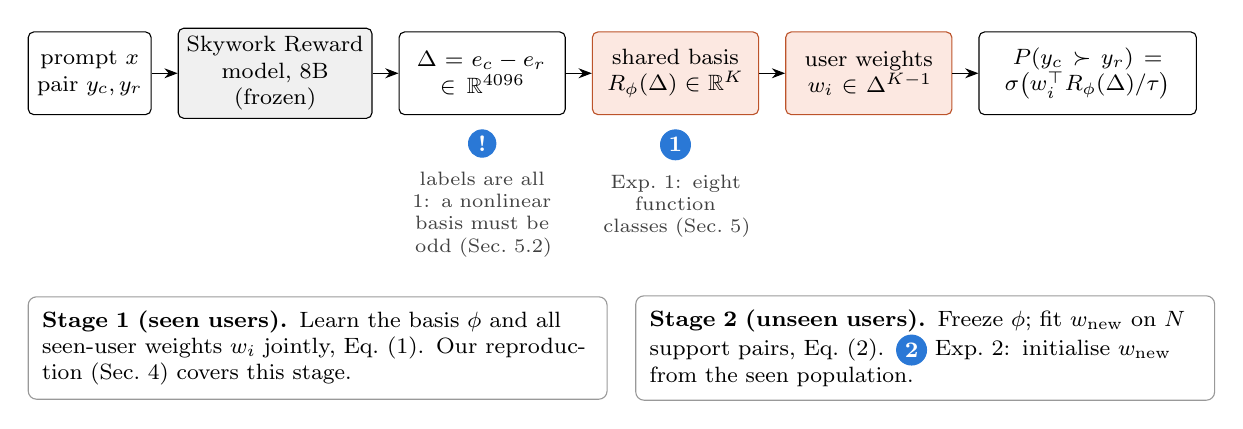
\begin{tikzpicture}[
  font=\footnotesize, >=Stealth, node distance=0.33cm,
  box/.style={draw, rounded corners=2pt, align=center, minimum height=1.05cm, inner sep=3pt, fill=white, text width=#1},
  box/.default=1.75cm,
  frozen/.style={box=#1, fill=gray!12},
  learn/.style={box=#1, fill=lorecol!15, draw=lorecol!80!black},
  probe/.style={circle, draw=basecol, fill=basecol, text=white, font=\bfseries\footnotesize, inner sep=1.3pt},
  note/.style={font=\scriptsize, text=black!75, align=center, text width=#1},
  stage/.style={draw=black!40, rounded corners=3pt, align=left, inner sep=5pt, font=\footnotesize, text width=7.0cm}
]
\node[box=1.35cm] (in) {prompt $x$\\pair $y_c,y_r$};
\node[frozen=2.25cm, right=of in] (enc) {Skywork Reward\\model, 8B\\(frozen)};
\node[box=1.9cm, right=of enc] (delta) {$\Delta=e_c-e_r$\\$\in\R^{4096}$};
\node[learn=1.9cm, right=of delta] (basis) {shared basis\\$R_\phi(\Delta)\in\R^{K}$};
\node[learn=1.9cm, right=of basis] (w) {user weights\\$w_i\in\Delta^{K-1}$};
\node[box=2.55cm, right=of w] (out) {$P(y_c\succ y_r)=$\\$\sigma\big(w_i^\top R_\phi(\Delta)/\tau\big)$};
\foreach \a/\b in {in/enc, enc/delta, delta/basis, basis/w, w/out} \draw[->] (\a) -- (\b);

\node[probe, below=0.18cm of delta] (p0) {!};
\node[note=2.3cm, below=0.06cm of p0] {labels are all 1: a nonlinear basis must be odd (Sec.~5.2)};
\node[probe, below=0.18cm of basis] (p1) {1};
\node[note=2.3cm, below=0.06cm of p1] {Exp.~1: eight function classes (Sec.~5)};

\node[stage, below=2.3cm of in.south west, anchor=north west] (s1)
  {\textbf{Stage 1 (seen users).} Learn the basis $\phi$ and all seen-user weights $w_i$ jointly, Eq.~(1). Our reproduction (Sec.~4) covers this stage.};
\node[stage, right=0.35cm of s1] (s2)
  {\textbf{Stage 2 (unseen users).} Freeze $\phi$; fit $w_\text{new}$ on $N$ support pairs, Eq.~(2).
  \tikz[baseline=-0.6ex]\node[probe]{2}; Exp.~2: initialise $w_\text{new}$ from the seen population.};
\end{tikzpicture}
\caption{The LoRe pipeline as we implemented it, and where each of our experiments intervenes. Grey: frozen;
orange: learned. Embeddings are extracted once and cached; all experiments then run on cached
4096-d vectors.}
\label{fig:schematic}
\end{figure}

\paragraph{Embeddings.} \Cref{fig:schematic} shows the pipeline. We extract the final-token last hidden
state of \texttt{Skywork-Reward-Llama-3.1-8B-v0.2} \citep{liu2024skywork} for the chat-formatted pair
[user: $x$, assistant: $y$] on an A100 in bf16. This gives 75{,}216\,+\,8{,}000 vectors for PersonalLLM
(9{,}402 / 1{,}000 prompts $\times$ 8 responses) and 28{,}280 for Reddit. Batched, right-padded inference
differs from single-sequence inference by a relative $L_2$ error of $10^{-2}$ (cosine 0.99995).

\paragraph{Benchmarks.} \textbf{PersonalLLM} \citep{zollo2024personalllm}: each response is scored by ten
reward models. A synthetic user is $w\sim\mathrm{Dir}(\alpha\mathbf{1}_{10})$, and for every sampled
prompt the best and worst of the eight responses under $w$ form the pair. We use 1{,}000 seen and 500
unseen users. Seen users get 47 training prompts and unseen users 9; all 1{,}000 test prompts are used
for evaluation, so each user is scored on 1{,}000 pairs. \textbf{Reddit TL;DR} \citep{stiennon2020learning}:
workers present in both splits are shuffled and halved, giving 20 seen and 19 unseen workers (one
worker with a single annotation is dropped). Seen workers contribute up to 100 or 150 comparisons and
unseen workers 50 few-shot comparisons. Evaluation uses up to 300 held-out comparisons per worker
(10{,}275 in total).

\paragraph{Training.} Unless stated otherwise we use $K=5$ basis functions and five seeds (42--46).
On PersonalLLM, stage~1 runs for 2{,}000 steps and stage~2 for 1{,}000. On Reddit, and for every basis in
Experiment~1, the step counts are 1{,}000 and 500.

% ======================================================================
\section{Reproducing LoRe}
\label{sec:repro}

\begin{figure}[t]
\centering
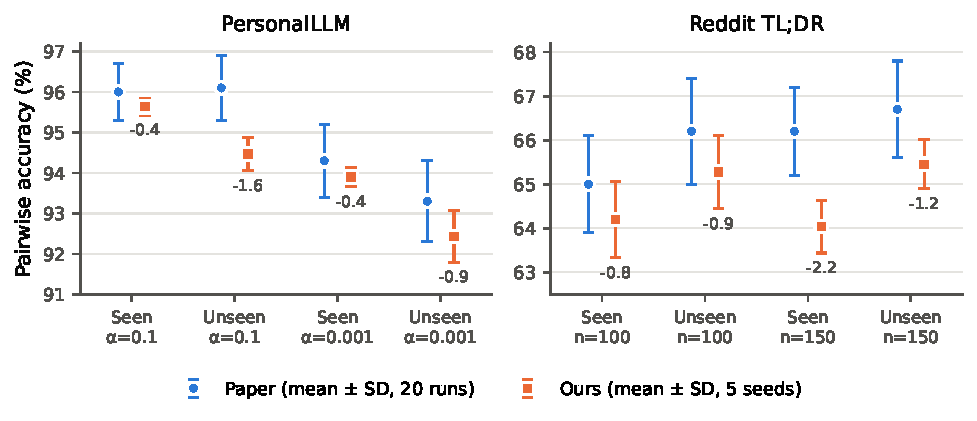
\includegraphics[width=\linewidth]{../figures/fig_reproduction.pdf}
\caption{Reproduction of LoRe (linear basis, $K=5$). Numbers under our points give our mean minus
the paper's mean. Error bars are the SD across runs. Dots rather than bars because the axis does not start at zero.}
\label{fig:repro}
\end{figure}

\begin{table}[t]
\centering\small
\caption{Reproduction results (mean $\pm$ SD across seeds, \%).}
\label{tab:repro}
\begin{tabular}{@{}llcccc@{}}
\toprule
Benchmark & Setting & Paper seen & Ours seen & Paper unseen & Ours unseen \\
\midrule
PersonalLLM & $\alpha=0.1$   & $96.0\pm0.7$ & $95.63\pm0.20$ & $96.1\pm0.8$ & $94.46\pm0.41$ \\
            & $\alpha=0.001$ & $94.3\pm0.9$ & $93.90\pm0.24$ & $93.3\pm1.0$ & $92.43\pm0.63$ \\
\midrule
Reddit TL;DR & $n=100$ & $65.0\pm1.1$ & $64.20\pm0.87$ & $66.2\pm1.2$ & $65.28\pm0.82$ \\
             & $n=150$ & $66.2\pm1.0$ & $64.03\pm0.60$ & $66.7\pm1.1$ & $65.45\pm0.55$ \\
\bottomrule
\end{tabular}
\end{table}

\Cref{fig:repro,tab:repro} compare our numbers with the paper. Every one of our means lies within
roughly two paper-SDs of the reported value. The ordering of settings is preserved: $\alpha=0.1$ is
easier than $\alpha=0.001$, and PersonalLLM is far easier than Reddit. We take this as a successful
reproduction and use it as the baseline for both experiments. Two details nevertheless differ:

\begin{itemize}
\item \textbf{Unseen is not better than seen on PersonalLLM.} The paper reports unseen accuracy \emph{at or above}
seen accuracy at $\alpha=0.1$ (96.1 vs 96.0), although unseen users have only 9 pairs against 47. In
our runs unseen accuracy is consistently lower ($-1.2$\pp), which is what one would expect. Our
few-shot fits reach 98.9\% \emph{training} accuracy on the 9 support pairs but 94.5\% on test pairs,
so the few-shot step overfits. The paper does not report few-shot training accuracy, which would have
exposed this overfitting. It motivates Experiment~2.
\item \textbf{More seen-user data does not help on Reddit.} Going from 100 to 150 examples per seen user
leaves overall accuracy unchanged (64.74\% in both cases; paired $t$-test on seen accuracy $p=0.71$). The
paper reports $+0.9$\pp. Per-user SDs are 3--10\pp with only 20 users per group, so most
between-method differences of about 1\pp in the paper's Reddit table are within noise.
\end{itemize}

% ======================================================================
\section{Experiment 1: changing the representation and the function class}
\label{sec:arch}

\paragraph{Motivation.} The paper uses a single linear map as the basis in every experiment, although it
suggests richer options (an MLP, or fine-tuning the encoder) without testing them. We want to know
whether the linear choice is a deliberate optimum or simply the first thing that worked, and whether an
even simpler basis would do.

\paragraph{Design.} We hold everything fixed except the basis $R_\phi$: $K=5$, the same optimiser and
temperature, the same splits (PersonalLLM $\alpha=0.1$; Reddit $n=150$) and five seeds. Every basis
takes the 4096-d difference $\Delta$ as input. We test:
\begin{enumerate}[label=\arabic*.]
\item \textbf{PCA-5}: the top-5 principal directions of the seen-user training differences, frozen.
Only the user weights are learned, so this tests whether the basis needs to be learned at all.
\item \textbf{PCA-512 + linear}: a frozen 512-d PCA projection followed by a learned $512\to5$ map.
\item \textbf{Random-512 + linear}: the same, but with a random orthonormal projection. Comparing it
with PCA-512 asks whether the compression has to be data-dependent.
\item \textbf{Linear (LoRe)}: $4096\to5$, no bias; the paper's basis (its Example~1).
\item \textbf{MLP-8} and \textbf{MLP-64}: two-layer GELU networks with 8 or 64 hidden units, a version of
the paper's Example~2. Both are made odd (\cref{sec:shortcut}).
\item \textbf{Residual-16}: the linear basis plus a rank-16 nonlinear residual branch, also made odd.
\item \textbf{Anchor + residual}: a prior-informed basis. Column 0 is the frozen Skywork reward direction
$a$ (its \texttt{score.weight}, so Skywork's own reward is $a^\top e$), with coefficient fixed to 1. Four
learned directions are kept orthogonal to $a$ and rescaled to $\|a\|$, and users mix only those four.
The hypothesis behind this basis is that everyone shares the reference reward and personalisation is a
correction on top of it.
\end{enumerate}
For reference we also report the frozen Skywork reward on its own, with no personalisation.

\paragraph{What we expect.} The fixed bases (PCA-5, and to a lesser extent the 512-d projections)
should \emph{underperform} the learned linear basis, because they cannot adapt their directions to what
users actually disagree about. The MLPs, the residual basis and the anchored basis should \emph{match or
slightly exceed} the linear basis. However, they have more trainable parameters than LoRe, and we do
\emph{not} expect a large jump in accuracy. The linear basis already performs well, and the paper's own
baselines (PAL and VPL, each with about 2.4M parameters) do not beat it despite far greater capacity.

\begin{figure}[t]
\centering
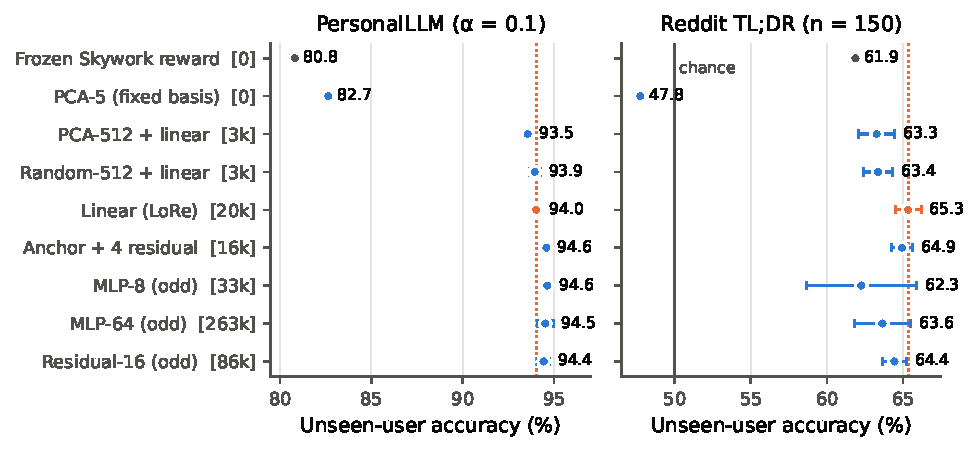
\includegraphics[width=\linewidth]{../figures/fig_architecture.pdf}
\caption{Unseen-user accuracy for each basis (mean $\pm$ SD over 5 seeds). Brackets give the
\emph{shared} trainable parameters of the basis; user weights add $5$ per user. The dotted line marks LoRe's linear basis.}
\label{fig:arch}
\end{figure}

\begin{table}[t]
\centering\small
\setlength{\tabcolsep}{4.2pt}
\caption{Function-class ablation (mean over 5 seeds, \%; seed SD for held-out columns). ``Train''
columns are the seen users' training pairs and the unseen users' few-shot support pairs (``--'': not logged). Best held-out
value per column in bold.}
\label{tab:arch}
\resizebox{\linewidth}{!}{%
\begin{tabular}{@{}lr cccc c cccc@{}}
\toprule
& & \multicolumn{4}{c}{\textbf{PersonalLLM} ($\alpha=0.1$)} && \multicolumn{4}{c}{\textbf{Reddit TL;DR} ($n=150$)}\\
\cmidrule{3-6}\cmidrule{8-11}
Basis & params & train & seen & few-shot & unseen && train & seen & few-shot & unseen\\
\midrule
Frozen Skywork & 0 & 83.6 & 83.33 & 81.4 & 80.82 && 60.4 & 63.10 & 63.4 & 61.87 \\
PCA-5 & 0 & 85.7 & 84.96\,{\scriptsize$\pm$0.00} & 85.7 & 82.65\,{\scriptsize$\pm$0.00} && 51.7 & 48.14\,{\scriptsize$\pm$0.03} & 56.2 & 47.75\,{\scriptsize$\pm$0.03}\\
PCA-512 + lin. & 2.6k & 99.3 & 95.06\,{\scriptsize$\pm$0.10} & 98.8 & 93.55\,{\scriptsize$\pm$0.17} && 99.4 & 60.41\,{\scriptsize$\pm$1.08} & 70.0 & 63.26\,{\scriptsize$\pm$1.18}\\
Rand-512 + lin. & 2.6k & 97.6 & 95.64\,{\scriptsize$\pm$0.08} & 98.0 & 93.94\,{\scriptsize$\pm$0.30} && 98.8 & 60.80\,{\scriptsize$\pm$0.29} & 71.7 & 63.36\,{\scriptsize$\pm$0.96}\\
\textcolor{lorecol}{\textbf{Linear (LoRe)}} & 20.5k & 99.4 & 95.87\,{\scriptsize$\pm$0.21} & 98.8 & 94.02\,{\scriptsize$\pm$0.24} && 99.7 & 64.19\,{\scriptsize$\pm$0.45} & 72.8 & \textbf{65.33}\,{\scriptsize$\pm$0.85}\\
Anchor + 4 res. & 16.4k & -- & \textbf{96.01}\,{\scriptsize$\pm$0.11} & -- & 94.58\,{\scriptsize$\pm$0.15} && -- & 64.31\,{\scriptsize$\pm$0.84} & -- & 64.93\,{\scriptsize$\pm$0.69}\\
MLP-8 (odd) & 32.8k & 100.0 & 95.80\,{\scriptsize$\pm$0.17} & 98.5 & \textbf{94.63}\,{\scriptsize$\pm$0.17} && 100.0 & \textbf{64.66}\,{\scriptsize$\pm$0.62} & 68.0 & 62.26\,{\scriptsize$\pm$3.61}\\
MLP-64 (odd) & 262.5k & 98.9 & 95.44\,{\scriptsize$\pm$0.33} & 97.7 & 94.52\,{\scriptsize$\pm$0.42} && 100.0 & 64.27\,{\scriptsize$\pm$0.43} & 69.5 & 63.64\,{\scriptsize$\pm$1.85}\\
Residual-16 (odd) & 86.1k & 100.0 & 95.58\,{\scriptsize$\pm$0.17} & 98.6 & 94.43\,{\scriptsize$\pm$0.31} && 100.0 & 64.36\,{\scriptsize$\pm$1.01} & 70.3 & 64.43\,{\scriptsize$\pm$0.78}\\
\bottomrule
\end{tabular}}
\end{table}

\subsection{Results: the linear basis is essentially sufficient}

\Cref{fig:arch,tab:arch} summarise the ablation. The expectations hold, with one surprise on Reddit.

\subsubsection*{Nonlinear bases buy little on PersonalLLM}
The best nonlinear basis, MLP-8, improves unseen accuracy by $+0.61$\pp over the linear basis (94.63
vs 94.02). The gain is statistically clear (Welch $p=0.002$) but small, and it comes at 1.6$\times$ the
shared parameters. MLP-64 and Residual-16 are not significantly better than linear ($p\approx0.05$).

\subsubsection*{On real users they are worse}
On Reddit every nonlinear basis loses unseen accuracy relative to linear, by 0.9 to 3.1\pp, and MLP-8
becomes unstable across seeds (unseen SD 3.6\pp, against 0.85 for linear). The training columns of
\cref{tab:arch} show why. \emph{Every} learned basis, linear included, fits the seen users' training
pairs to 99--100\% but generalises at only 60--65\%. Capacity is therefore not the bottleneck on
Reddit; label noise and the small number of pairs per user are, and extra capacity can only be spent
on memorisation.

\subsubsection*{Compression helps little, and it does not need to be learned}
A \emph{random} 512-d projection is as good as PCA-512: slightly better on PersonalLLM ($93.94$ vs
$93.55$, $p=0.04$) and indistinguishable on Reddit ($p=0.89$). With 8$\times$ fewer trainable parameters
than LoRe, it loses only 0.1\pp on PersonalLLM (not significant, $p=0.67$) but 2\pp on Reddit
($p=0.009$). The variance structure agrees: the top five principal components explain 66\% of the
variance of difference vectors on PersonalLLM but only 42\% on Reddit, so real preferences are spread
over more directions of the embedding.

\subsubsection*{Fixed bases underperform, as expected}
PCA-5, which has no learned basis, gets 82.7\% on PersonalLLM, barely above the frozen Skywork reward.
On Reddit it scores 47.8\%, which is \emph{below chance}; \cref{sec:simplex} investigates why.

\subsubsection*{The pre-trained reward direction is a useful prior}
The anchored basis is the best model for seen users on PersonalLLM (96.01\%), and it is within noise of
the best on unseen users on both benchmarks, with fewer shared parameters than LoRe (16.4k vs 20.5k).
LoRe initialises $A$ randomly and so discards the one direction the reward model was trained to
encode. Anchoring keeps that direction for free, and it makes the basis interpretable: each user is
``Skywork plus a personal correction''.

\subsection{An unexpected 100\% accuracy: the orientation shortcut}
\label{sec:shortcut}

Our first implementation of MLP-8, MLP-64 and Residual-16 used ordinary two-layer networks, with bias
terms, applied directly to the cached difference vectors $\Delta$. All three reached \textbf{100.00\%}
accuracy on both seen and unseen users, on both benchmarks, with the training loss driven to zero and
no variation across users. On Reddit, where no linear model we trained exceeded about 66\% because the
annotator labels are noisy, a perfect score is not plausible. We therefore treated it as a symptom to
explain, not a result to report.

The explanation lies in how the training data is presented. Every pair is stored as
$\Delta=e(x,y_c)-e(x,y_r)$, chosen minus rejected, so every training label is 1 and the model never
sees a pair in the opposite orientation. A network with an output bias can represent a constant
function $f(\Delta)\equiv c$. If $w^\top c>0$, the margin $w^\top f(\Delta)/\tau$ is positive for every
input, and by scaling $c$ the loss
\[
\sum_j \ell\!\left(w^\top f(\Delta_j)/\tau\right)
\]
can be driven arbitrarily close to zero without using any information in $\Delta$. Because the test
pairs are stored in the same orientation, such a function is also ``correct'' on every test pair,
which is exactly the 100\% we observed. In effect, the networks could learn the answer key (``the first
response always wins'') instead of the users' preferences.

This diagnosis suggests a simple sanity check: score every test pair in both orientations. Presenting
$-\Delta$ describes the same comparison with the two responses swapped, so its correct label is 0 and
the prediction should flip. A constant-output model predicts ``first wins'' in both orientations, so on
this symmetrised test set it is right exactly half the time, 50\%. A genuine preference model is
unaffected, provided it is \emph{odd}, $f(-\Delta)=-f(\Delta)$. Then $w^\top f(-\Delta)=-w^\top f(\Delta)$,
so the swapped pair is classified correctly exactly when the original is, and the standard and swapped
accuracies coincide.

The same reasoning explains why LoRe itself never meets the problem. A bias-free linear map is odd,
$A(-\Delta)=-A\Delta$, so precomputing differences is harmless for the paper's linear basis. It also
explains why the paper's ``Example~2'' applies the MLP to each embedding separately: the margin
$f(e_c)-f(e_r)$ changes sign automatically when the responses are swapped. The shortcut appears only
when a nonlinear map is applied to a precomputed difference, which is a natural optimisation once
embeddings are cached in that form.

Our correction was to antisymmetrise each nonlinear basis,
\[
f_\text{odd}(\Delta)=\tfrac12\big(f(\Delta)-f(-\Delta)\big),
\]
which is odd by construction. A constant component now cancels exactly, $\tfrac12(c-c)=0$, so the
shortcut is no longer available, and the accuracies returned to the plausible range reported in
\cref{tab:arch}. All nonlinear results in this report use this form. The antisymmetrised network is a
valid \emph{pairwise} model, but it is not a per-response reward model, so it cannot guarantee
transitive rankings over three or more responses; this is a further argument for the linear basis.
More generally, we recommend reporting swapped-pair accuracy alongside standard accuracy whenever a
nonlinear model is trained on difference vectors. It costs one extra forward pass and exposes this
failure immediately.

\subsection{A below-chance basis: PCA-5 on Reddit}
\label{sec:simplex}

PCA-5 is the only basis with nothing to learn in the basis itself. Its directions are the top five
principal components of the seen users' training differences, and only the user weights are fitted.
On PersonalLLM it reaches 82.7\%, slightly above the frozen Skywork reward. On Reddit, however, it
scores 47.8\% on unseen users (48.1\% on seen users), below chance. With a seed SD of only 0.00--0.03\pp,
the shortfall is systematic, not noise.

A model that falls below chance is consistently ranking the wrong response higher, so we examined what
this model can and cannot express. With fixed basis directions $p_1,\dots,p_K$, a user's score for a
pair is
\[
s_w(\Delta)=\sum_{k=1}^{K} w_k\,p_k^\top\Delta,\qquad w\in\simplex .
\]
Because the weights are non-negative and sum to one, $s_w(\Delta)$ is a convex combination, i.e.\ a
weighted average, of the $K$ projections $p_k^\top\Delta$. A weighted average of negative numbers is
negative. On any pair where \emph{every} projection has the wrong sign, the model is therefore wrong
for every possible choice of $w$, and no amount of fitting the user's weights can repair it. If a
fraction $\rho$ of pairs are of this kind, accuracy is at most $1-\rho$ whatever the user's weights,
and once $\rho>\tfrac12$ the model is necessarily below chance.

Why would a PCA basis produce many such pairs? Principal components are defined only up to sign: $v$
and $-v$ are equally valid eigenvectors, and which one the solver returns bears no relation to which
direction users prefer. A learned basis is unaffected, because training can flip any direction of $A$.
Simplex weights cannot: a user can down-weight a wrong-signed direction, but can never \emph{negate}
it. On PersonalLLM the top five components explain 66\% of the variance and this evidently costs
little. On Reddit they explain only 42\% and the preference signal is weak, so a basis whose
components happen to point mostly against users' preferences would produce exactly the behaviour we
see. We did not measure $\rho$ directly, so we present this as the most plausible mechanism, not an
established cause. The near-zero seed variance fits the same picture. With the basis fixed, the
objective is convex in $w$, and every seed converged to essentially the same accuracy.

The practical implication is that a fixed or externally supplied basis should not be combined with
simplex weights as-is. It needs either unconstrained weights $w\in\R^K$ or a sign-symmetric basis
$\{\pm p_k\}$ that lets a user express both orientations of every direction.

% ======================================================================
\section{Experiment 2: how should a new user be initialised?}
\label{sec:init}

\paragraph{Motivation.} LoRe fits a new user from $\theta\sim\mathcal{N}(0,I)$, ignoring the 1{,}000 seen
users it has just learned. At deployment the per-user step must be cheap, and the reproduction showed
that it overfits with 9 pairs. We therefore ask whether the seen population can supply a better starting
point, and how much that matters.

\paragraph{Design.} We reuse the five PersonalLLM ($\alpha=0.1$) bases from the reproduction and verified
that re-evaluating their saved weights reproduces the original unseen accuracies to within $10^{-5}$\pp.
For each of the 500 unseen users we build \emph{nested} support sets of $N\in\{5,15,50,150\}$ pairs. The
original 9 prompts come first and are extended with new prompts; the query set is all 1{,}000 test
prompts. We compare five starting points:
\begin{enumerate}[label=\arabic*.]
\item \textbf{Random logits}: LoRe's default.
\item \textbf{Uniform}: $w=\mathbf{1}/K$.
\item \textbf{Population mean}: the average of the learned seen-user weights.
\item \textbf{Nearest seen user}: the seen user's $w$ with the lowest BT loss on the new user's support set.
\item \textbf{Cluster centroid}: the best of five $k$-means centroids of the seen-user weights, also
chosen by support loss.
\end{enumerate}
The last two use the support data only to \emph{select} among existing weight vectors; they do not
optimise. From each start we run 0, 5, 20 or 50 Adam updates (lr 0.1).

\paragraph{What we expect.} We try different initialisations to see whether a new user can be fitted
with fewer support examples, and how quickly (in gradient steps) the fit adapts. The selected starts,
nearest seen user and cluster centroid, should be strong starting points, since a new user is likely to
resemble someone already in the population. The population mean averages over users who disagree, and
a random start carries no information at all. With a sufficient number of support examples and
sufficient gradient steps, however, we expect all initialisations to perform similarly. With the basis
frozen, the few-shot objective is convex in $w$, so the starting point should mainly affect how quickly
the optimiser approaches a good solution, not where it ends up. The open questions are how large the
early advantage is, how long it lasts, and whether a good start still helps when support examples are scarce.

\begin{figure}[t]
\centering
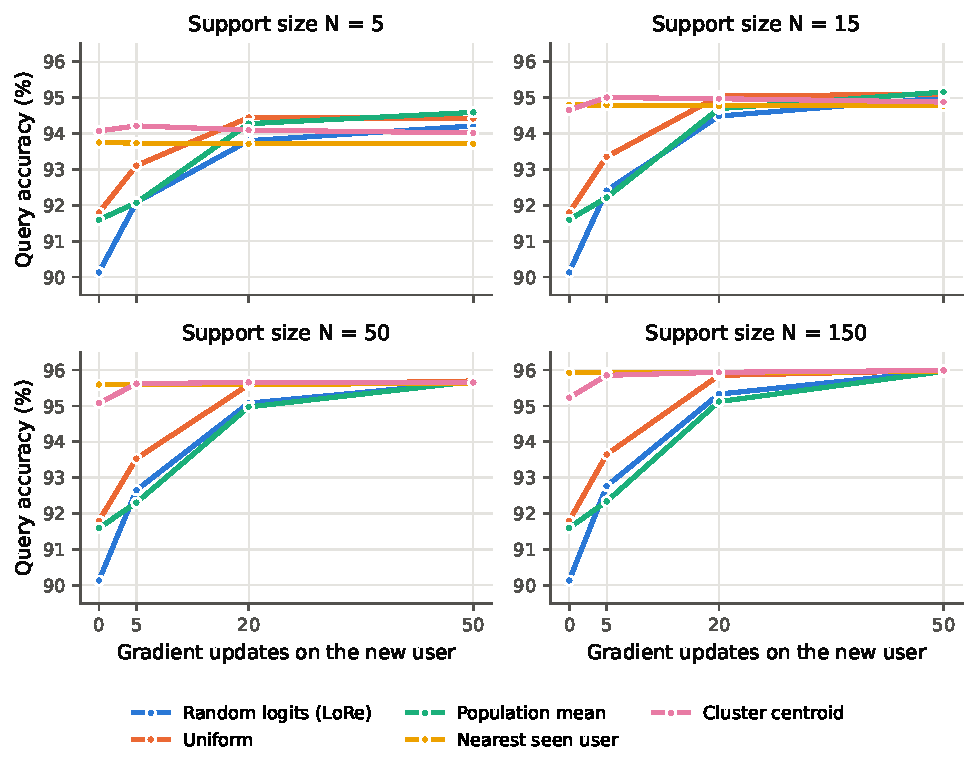
\includegraphics[width=\linewidth]{../figures/fig_init_curves.pdf}
\caption{Query accuracy of unseen users against the number of few-shot updates, for five
initialisations and four support sizes (mean of 5 seeds; seed SDs are 0.2--0.7\pp).}
\label{fig:init}
\end{figure}

\begin{table}[t]
\centering\small
\caption{Paired improvement over LoRe's random-logit start (pp, mean over 5 seeds, 95\% $t$-interval
in brackets).}
\label{tab:init}
\setlength{\tabcolsep}{4pt}
\begin{tabular}{@{}lccccc@{}}
\toprule
& & \multicolumn{4}{c}{Gradient updates} \\
\cmidrule{3-6}
Initialisation & $N$ & 0 & 5 & 20 & 50\\
\midrule
Uniform & 15 & $+1.67$ {\scriptsize[1.21, 2.12]} & $+0.94$ {\scriptsize[0.55, 1.34]} & $+0.56$ {\scriptsize[0.42, 0.69]} & $+0.11$ {\scriptsize[0.03, 0.18]}\\
Population mean & 15 & $+1.47$ {\scriptsize[0.89, 2.04]} & $-0.19$ {\scriptsize[$-$0.67, 0.29]} & $+0.21$ {\scriptsize[$-$0.12, 0.54]} & $+0.16$ {\scriptsize[0.07, 0.26]}\\
Nearest seen user & 15 & $+4.67$ {\scriptsize[3.73, 5.61]} & $+2.38$ {\scriptsize[1.98, 2.79]} & $+0.29$ {\scriptsize[0.06, 0.51]} & $-0.22$ {\scriptsize[$-$0.42, $-$0.02]}\\
Cluster centroid & 15 & $+4.53$ {\scriptsize[4.00, 5.05]} & $+2.60$ {\scriptsize[2.23, 2.96]} & $+0.49$ {\scriptsize[0.32, 0.65]} & $-0.12$ {\scriptsize[$-$0.31, 0.07]}\\
\midrule
Nearest seen user & 50 & $+5.46$ {\scriptsize[4.53, 6.39]} & $+2.96$ {\scriptsize[2.57, 3.35]} & $+0.53$ {\scriptsize[0.38, 0.67]} & $-0.04$ {\scriptsize[$-$0.08, $-$0.01]}\\
Cluster centroid & 50 & $+4.95$ {\scriptsize[4.36, 5.54]} & $+2.97$ {\scriptsize[2.58, 3.35]} & $+0.58$ {\scriptsize[0.43, 0.74]} & $-0.02$ {\scriptsize[$-$0.07, 0.03]}\\
\midrule
Nearest seen user & 150 & $+5.79$ {\scriptsize[4.82, 6.76]} & $+3.16$ {\scriptsize[2.71, 3.61]} & $+0.60$ {\scriptsize[0.43, 0.77]} & $-0.02$ {\scriptsize[$-$0.04, $-$0.01]}\\
Cluster centroid & 150 & $+5.10$ {\scriptsize[4.43, 5.76]} & $+3.09$ {\scriptsize[2.67, 3.50]} & $+0.61$ {\scriptsize[0.42, 0.80]} & $+0.01$ {\scriptsize[$-$0.01, 0.02]}\\
\bottomrule
\end{tabular}
\end{table}

\paragraph{Results.} \Cref{fig:init,tab:init} confirm the main expectations: selected starts are much
better at first, and with enough data everything converges later.
\begin{itemize}
\item \textbf{Large gains at small budgets.} With no gradient steps at all, selecting a seen user or a
centroid by support loss improves query accuracy over LoRe's start by $+4.5$ to $+5.8$\pp. After 5
updates the gain is still $+2.4$ to $+3.2$\pp, with all five seeds positive in every setting.
\item \textbf{Convergence with enough data.} By 50 updates the five strategies differ by at most 0.07\pp for
$N\ge50$, against gaps of up to 5.8\pp at the start. With smaller supports the remaining spread is 0.4\pp ($N=15$)
and 0.9\pp ($N=5$), because there the selected starts overfit (next point). This is consistent with the convexity of the
few-shot objective: here, initialisation buys speed, not a better optimum.
\item \textbf{A lookup can replace the optimisation.} \Cref{fig:zero} compares zero-update selection with
fully adapted baselines. For $N\ge50$ the nearest seen user with \emph{no} updates is within 0.08\pp of
50 steps of LoRe's adaptation (95.59 vs 95.67 at $N=50$; 95.92 vs 95.98 at $N=150$). At $N=5$ the
cluster centroid with zero updates (94.07\%) is statistically indistinguishable from 50 random-start
updates (94.21\%, 95\% CI of the difference $[-0.67, 0.39]$). Selection costs one $N\times K$ matrix
product against 1{,}000 candidates, with no backward passes.
\item \textbf{With tiny support sets, more optimisation hurts.} At $N=5$ and $N=15$ the selected
starts \emph{lose} accuracy as updates continue (e.g.\ cluster centroid 94.21$\to$94.02 at $N=5$), and
the uniform start peaks at 20 updates. With 5 pairs and 5 free parameters the empirical minimiser
overfits. Choosing a point on the seen-population manifold acts as a regulariser, much like a MAP
estimate under a population prior. Early stopping, or an explicit penalty towards the selected
prior, would be the principled fix.
\item \textbf{The population mean is a poor prior.} It is worse than uniform after 5 updates by 1.0
to 1.3\pp, because the mean of a diverse ($\alpha=0.1$) population sits between clusters and
represents nobody. Personalisation needs selection, not averaging.
\item \textbf{No long-run benefit when examples are scarce.} We had hoped that the population-informed
starts would also yield a better \emph{final} model when support examples are few, with the selected
weights acting as a prior that gradient updates refine. We did not see this. At $N=5$ and $N=15$, after
50 updates the nearest-seen-user and cluster-centroid starts are no better than the random or uniform
starts (at $N=15$: $-0.22$ and $-0.12$\pp relative to random logits; at $N=5$: 94.02\% for the cluster
centroid against 94.21\% for random logits). Their advantage is confined to the first few updates.
\end{itemize}

\begin{figure}[t]
\centering
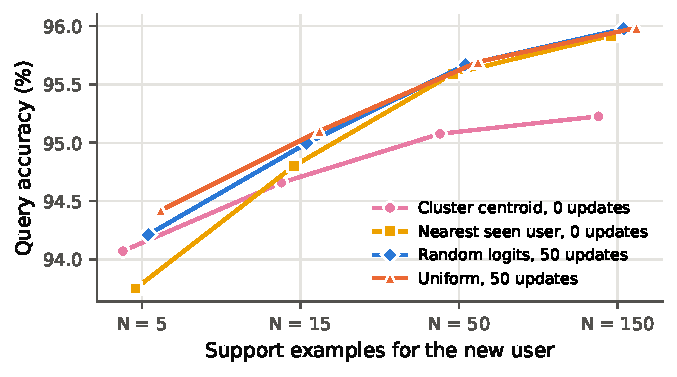
\includegraphics[width=0.68\linewidth]{../figures/fig_zero_update.pdf}
\caption{Zero-update selection (circles, squares) against 50 updates of gradient adaptation from the
random and uniform starts (diamonds, triangles). The cluster centroid is limited by having only five
candidates; the nearest seen user keeps up as $N$ grows.}
\label{fig:zero}
\end{figure}

% ======================================================================
\section{Discussion: what we learned about LoRe}
\label{sec:discussion}

\paragraph{Answer to the central question.} LoRe's personalisation comes from the \emph{low-rank shared
structure} learned on a good frozen representation, not from the expressivity of the basis. Within the
model, the three components play very different roles:
(1)~the \textbf{basis function class} is close to saturated already at linear. Simpler bases lose
accuracy on real users, richer ones only memorise, and the most useful change is to keep the
pre-trained reward direction;
(2)~the \textbf{simplex constraint} is harmless when the basis is learned, but it becomes a real
restriction for a fixed basis (\cref{sec:simplex});
(3)~the \textbf{few-shot optimisation} is the least essential component. Given enough data and updates, its outcome
does not depend on the starting point, and choosing among the seen users' weights gets there with no
optimisation at all.

\paragraph{Critique of the paper.}
\begin{itemize}
\item \textbf{The semi-synthetic benchmark matches LoRe's own model class.} PersonalLLM users are exact
linear mixtures of ten reward models, and those models are close to linear in a strong reward model's
embedding. LoRe's large margin there (Table~1 of the paper) therefore says more about matched
inductive bias than about personalising real users.
\item \textbf{The design choices are not ablated}, and two training details that matter are not stated:
the temperature $\tau=100$ and the learning rate of 0.5. The rank $B$ is chosen by cross-validation
over a wide grid, which slightly flatters LoRe relative to baselines run with default settings.
\item \textbf{Statistical resolution.} With 20 users per group and per-user SDs of 3--10\pp, many of the
roughly 1\pp differences in the paper's Reddit table are not resolvable. The unseen-above-seen pattern
on PersonalLLM did not replicate in our runs.
\end{itemize}

\section{Limitations}
We used five seeds instead of twenty and $K=5$ throughout instead of a cross-validated rank. Reddit
was evaluated on a 300-pair-per-worker subsample, and PRISM was not reproduced. Experiment~2 uses only
PersonalLLM at $\alpha=0.1$, where seen-user clusters are well defined because the users are synthetic.
On real users the benefit of selection may be smaller. Seed SDs for the $N=5$ and $N=15$ conditions were
not recorded per method, so for those we report paired intervals only where available. The embedding
extraction and all training ran on a single GPU, which ruled out fine-tuning the encoder (the paper's
Example~3).

\section{Conclusion}
We reproduced LoRe and then took it apart. Its accuracy rests on a shared low-rank structure over a
strong frozen representation. A plain linear basis already captures what that representation offers:
nonlinear bases add at most 0.6\pp on synthetic users and nothing on real ones. Along the way we found
and explained a pitfall: nonlinear bases on precomputed differences admit a 100\%-accuracy shortcut
unless they are odd. Finally, a new user's initialisation mattered mainly before convergence; before convergence, however, it matters a great deal. Picking the
best-fitting seen user is as good as LoRe's 50-step adaptation and needs no gradient steps.

\paragraph{Code and results.} All experiments were run on Google Colab (A100). Code, per-seed results
and figure scripts are at \url{\repourl}; every number in this report is in \texttt{results/}.

\paragraph{Use of AI tools.} We have used AI to write code for the experiments, but we came up with the
ideas. We have also used AI to structure the report and correct and polish sentences.

% ======================================================================
\begin{thebibliography}{99}\small
\bibitem{bose2025lore} A.~Bose, Z.~Xiong, Y.~Chi, S.~S.~Du, L.~Xiao, M.~Fazel. LoRe: Personalizing LLMs via low-rank reward modeling. \emph{arXiv:2504.14439}, 2025.
\bibitem{bradley1952rank} R.~A.~Bradley, M.~E.~Terry. Rank analysis of incomplete block designs: I. The method of paired comparisons. \emph{Biometrika}, 39(3/4):324--345, 1952.
\bibitem{christiano2017deep} P.~F.~Christiano, J.~Leike, T.~Brown, M.~Martic, S.~Legg, D.~Amodei. Deep reinforcement learning from human preferences. \emph{NeurIPS}, 2017.
\bibitem{koren2009matrix} Y.~Koren, R.~Bell, C.~Volinsky. Matrix factorization techniques for recommender systems. \emph{Computer}, 42(8):30--37, 2009.
\bibitem{park2015preference} D.~Park, J.~Neeman, J.~Zhang, S.~Sanghavi, I.~Dhillon. Preference completion: Large-scale collaborative ranking from pairwise comparisons. \emph{ICML}, 2015.
\bibitem{chen2024pal} D.~Chen, Y.~Chen, A.~Rege, R.~K.~Vinayak. PAL: Pluralistic alignment framework for learning from heterogeneous preferences. \emph{arXiv:2406.08469}, 2024.
\bibitem{poddar2024vpl} S.~Poddar, Y.~Wan, H.~Ivison, A.~Gupta, N.~Jaques. Personalizing reinforcement learning from human feedback with variational preference learning. \emph{arXiv:2408.10075}, 2024.
\bibitem{liu2024skywork} C.~Y.~Liu, L.~Zeng, J.~Liu, R.~Yan, J.~He, C.~Wang, S.~Yan, Y.~Liu, Y.~Zhou. Skywork-Reward: Bag of tricks for reward modeling in LLMs. \emph{arXiv:2410.18451}, 2024.
\bibitem{zollo2024personalllm} T.~P.~Zollo, A.~W.~T.~Siah, N.~Ye, A.~Li, H.~Namkoong. PersonalLLM: Tailoring LLMs to individual preferences. \emph{arXiv:2409.20296}, 2024.
\bibitem{stiennon2020learning} N.~Stiennon, L.~Ouyang, J.~Wu, D.~Ziegler, R.~Lowe, C.~Voss, A.~Radford, D.~Amodei, P.~F.~Christiano. Learning to summarize with human feedback. \emph{NeurIPS}, 2020.
\bibitem{kirk2024prism} H.~R.~Kirk et~al. The PRISM alignment project. \emph{arXiv:2404.16019}, 2024.
\end{thebibliography}

% ======================================================================
\clearpage
\appendix
\section{Training configuration and reproduction per seed}
\label{app:details}

\begin{table}[ht]
\centering\small
\caption{Training configuration (shared by all experiments unless noted).}
\resizebox{\linewidth}{!}{%
\begin{tabular}{@{}ll@{}}
\toprule
Embedding model & Skywork-Reward-Llama-3.1-8B-v0.2, rev.\ \texttt{67e958f}, final-token hidden state, bf16\\
Basis rank $K$ & 5 (anchor basis: 1 fixed + 4 learned)\\
User weights & $w=\mathrm{softmax}(\theta)$, $\theta_0\sim\mathcal{N}(0,I)$\\
Temperature $\tau$ & 100\\
Joint stage & full-batch Adam, lr 0.5; 2{,}000 steps (reproduction, PersonalLLM), 1{,}000 (Reddit, Exp.~1)\\
Few-shot stage & full-batch Adam, lr 0.1; 1{,}000 steps (reproduction, PersonalLLM), 500 (Reddit, Exp.~1), $\le$50 (Exp.~2)\\
Loss & sum over users of per-user mean logistic loss\\
Projections & PCA (randomised SVD, seen-user training $\Delta$ only); random: QR of Gaussian, seed 42\\
Seeds & 42, 43, 44, 45, 46\\
\bottomrule
\end{tabular}}
\end{table}

\begin{table}[ht]
\centering\small
\caption{Per-seed reproduction results (\%).}
\begin{tabular}{@{}c cc cc c cc cc@{}}
\toprule
& \multicolumn{4}{c}{PersonalLLM} && \multicolumn{4}{c}{Reddit TL;DR}\\
\cmidrule{2-5}\cmidrule{7-10}
& \multicolumn{2}{c}{$\alpha=0.1$} & \multicolumn{2}{c}{$\alpha=0.001$} && \multicolumn{2}{c}{$n=100$} & \multicolumn{2}{c}{$n=150$}\\
Seed & seen & unseen & seen & unseen && seen & unseen & seen & unseen\\
\midrule
42 & 95.30 & 94.22 & 93.84 & 91.64 && 64.79 & 65.13 & 64.06 & 65.03\\
43 & 95.69 & 94.50 & 94.29 & 92.54 && 64.62 & 65.33 & 63.28 & 65.79\\
44 & 95.79 & 93.94 & 93.67 & 92.03 && 64.57 & 65.41 & 64.80 & 65.17\\
45 & 95.79 & 95.01 & 93.76 & 92.62 && 64.33 & 66.41 & 64.39 & 66.27\\
46 & 95.60 & 94.64 & 93.92 & 93.31 && 62.67 & 64.10 & 63.65 & 65.01\\
\bottomrule
\end{tabular}
\end{table}

\clearpage

\section{Experiment 1: per-seed results and parameter accounting}
\label{app:arch}
\Cref{tab:arch-seeds} shows that the large Reddit SD of MLP-8 comes from a single seed (seed 45, 56.0\%),
while the linear basis stays between 64.0 and 66.1\% on every seed. \Cref{tab:params} lists the parameter
counts behind \cref{fig:arch}.

\begin{table}[ht]
\centering\small
\caption{Experiment 1, per-seed unseen-user accuracy (\%). Per-seed values for the anchored basis were not
logged individually; its mean $\pm$ SD is in \cref{tab:arch}.}
\label{tab:arch-seeds}
\begin{tabular}{@{}l ccccc c ccccc@{}}
\toprule
& \multicolumn{5}{c}{PersonalLLM ($\alpha=0.1$), seed} && \multicolumn{5}{c}{Reddit TL;DR ($n=150$), seed}\\
\cmidrule{2-6}\cmidrule{8-12}
Basis & 42 & 43 & 44 & 45 & 46 && 42 & 43 & 44 & 45 & 46\\
\midrule
PCA-5 & 82.66 & 82.65 & 82.66 & 82.65 & 82.65 &  & 47.73 & 47.75 & 47.75 & 47.80 & 47.75\\
PCA-512 + linear & 93.82 & 93.42 & 93.54 & 93.40 & 93.55 &  & 63.60 & 61.98 & 62.52 & 63.15 & 65.06\\
Random-512 + linear & 94.17 & 93.62 & 93.72 & 93.89 & 94.32 &  & 63.17 & 63.82 & 64.75 & 62.29 & 62.77\\
Linear (LoRe) & 93.64 & 94.06 & 94.21 & 93.97 & 94.22 &  & 64.89 & 65.69 & 65.93 & 66.10 & 64.04\\
MLP-8 (odd) & 94.37 & 94.77 & 94.57 & 94.77 & 94.68 &  & 64.09 & 63.28 & 65.08 & 55.99 & 62.83\\
MLP-64 (odd) & 94.38 & 94.77 & 94.53 & 93.92 & 95.03 &  & 66.31 & 63.36 & 64.22 & 63.06 & 61.22\\
Residual-16 (odd) & 94.28 & 94.03 & 94.88 & 94.50 & 94.44 &  & 64.11 & 64.18 & 63.44 & 65.30 & 65.14\\
\bottomrule
\end{tabular}
\end{table}

\begin{table}[ht]
\centering\small
\caption{Experiment 1, parameter accounting. \emph{Shared}: trainable basis parameters. \emph{Total
trainable}: shared plus user weights (1{,}500 users on PersonalLLM, 39 on Reddit). \emph{Deployed}: everything
stored at inference, including frozen projections and the anchor.}
\label{tab:params}
\begin{tabular}{@{}l r rr c rr@{}}
\toprule
& & \multicolumn{2}{c}{PersonalLLM} && \multicolumn{2}{c}{Reddit TL;DR}\\
\cmidrule{3-4}\cmidrule{6-7}
Basis & Shared & Total trainable & Deployed && Total trainable & Deployed\\
\midrule
Frozen Skywork & 0 & 0 & 4{,}096 && 0 & 4{,}096\\
PCA-5 & 0 & 7{,}500 & 27{,}980 && 195 & 20{,}675\\
PCA-512 + linear & 2{,}560 & 10{,}060 & 2{,}107{,}212 && 2{,}755 & 2{,}099{,}907\\
Random-512 + linear & 2{,}560 & 10{,}060 & 2{,}107{,}212 && 2{,}755 & 2{,}099{,}907\\
Linear (LoRe) & 20{,}480 & 27{,}980 & 27{,}980 && 20{,}675 & 20{,}675\\
Anchor + 4 residual & 16{,}384 & 22{,}384 & 26{,}480 && 16{,}540 & 20{,}636\\
MLP-8 (odd) & 32{,}821 & 40{,}321 & 40{,}321 && 33{,}016 & 33{,}016\\
MLP-64 (odd) & 262{,}533 & 270{,}033 & 270{,}033 && 262{,}728 & 262{,}728\\
Residual-16 (odd) & 86{,}096 & 93{,}596 & 93{,}596 && 86{,}291 & 86{,}291\\
\bottomrule
\end{tabular}
\end{table}

\section{Experiment 2: absolute accuracies}
\label{app:init}
\Cref{tab:init} in the main text reports paired improvements over random logits; \cref{tab:init-abs} gives
the underlying absolute accuracies for every condition, including $N=5$.

\begin{table}[ht]
\centering\small
\caption{Experiment 2, absolute query accuracy of unseen users (\%, mean over 5 seeds) for every support
size $N$, initialisation and number of updates. Best value per column within each $N$ in bold.
$^\dagger$Derived from the paired-difference table (uniform minus its improvement over random logits).}
\label{tab:init-abs}
\begin{tabular}{@{}ll cccc@{}}
\toprule
& & \multicolumn{4}{c}{Gradient updates}\\
\cmidrule{3-6}
$N$ & Initialisation & 0 & 5 & 20 & 50\\
\midrule
\multirow{5}{*}{5} & Random logits (LoRe) & 90.13 & 92.08 & 93.80 & 94.21\\
 & Uniform & 91.80 & 93.11 & \textbf{94.44} & 94.42\\
 & Population mean & 91.60 & 92.07 & 94.27 & \textbf{94.59}\\
 & Nearest seen user & 93.75 & 93.73 & 93.71 & 93.71\\
 & Cluster centroid & \textbf{94.07} & \textbf{94.21} & 94.10 & 94.02\\
\midrule
\multirow{5}{*}{15} & Random logits (LoRe) & 90.13 & 92.41 & 94.49 & 95.00\\
 & Uniform & 91.80 & 93.35 & \textbf{95.04} & 95.10\\
 & Population mean & 91.60 & 92.22 & 94.69 & \textbf{95.16}\\
 & Nearest seen user & \textbf{94.80} & 94.79 & 94.77 & 94.78\\
 & Cluster centroid & 94.66 & \textbf{95.00} & 94.97 & 94.88\\
\midrule
\multirow{5}{*}{50} & Random logits (LoRe)$^\dagger$ & 90.13 & 92.65 & 95.07 & 95.67\\
 & Uniform & 91.80 & 93.53 & 95.59 & \textbf{95.69}\\
 & Population mean & 91.60 & 92.30 & 94.97 & 95.68\\
 & Nearest seen user & \textbf{95.59} & 95.61 & 95.60 & 95.62\\
 & Cluster centroid & 95.08 & \textbf{95.61} & \textbf{95.66} & 95.65\\
\midrule
\multirow{5}{*}{150} & Random logits (LoRe)$^\dagger$ & 90.13 & 92.76 & 95.33 & 95.98\\
 & Uniform & 91.80 & 93.64 & 95.85 & \textbf{95.99}\\
 & Population mean & 91.60 & 92.34 & 95.12 & 95.96\\
 & Nearest seen user & \textbf{95.92} & \textbf{95.92} & 95.93 & 95.96\\
 & Cluster centroid & 95.23 & 95.85 & \textbf{95.94} & \textbf{95.99}\\
\bottomrule
\end{tabular}
\end{table}


\end{document}
